\chapter{Implementación} \label{diseño}

A continuación se procederá a explicar la implementación de las funcionalidades más representativas dentro del sistema, explicando su lógica, flujo y estructura. Además, se hará una presentación de las herramientas que han complementado el desarrollo de la aplicación de forma profesional y eficiente.

\section{Herramientas}

Durante todo el ciclo de vida del proyecto se han utilizado diversas herramientas que han complementado las distintas fases del desarrollo, desde la construcción de código hasta la integración continua (CI/CD), control de versiones y contenedorización.

\subsection{VSCode IDE}
\begin{figure}[H]
  \centering
  
\includegraphics[width=0.2\textwidth]{fotos/vs.png}
  \caption{Logo IDE VSCode}
\end{figure}
Como entorno de desarrollo integrado (IDE) se ha utilizado Visual Studio Code (VSCode), un editor de código fuente desarrollado por Microsoft \cite{vscode}. VSCode ha sido escogido por el gran número de extensiones gratuitas que ofrece, permitiendo trabajar con múltiples tecnologías y lenguajes de programación simultáneamente. Su integración con sistemas de control de versiones(GitHub) y herramientas de desarrollo lo convierte en una gran opción para proyectos software profesionales.

\subsection{GitHub}
\begin{figure}[H]
  \centering
  
\includegraphics[width=0.3\textwidth]{fotos/git.png}
  \caption{Logo GitHub}
\end{figure}
GitHub ha desempeñado un papel central durante el desarrollo del proyecto, no solo como plataforma de control de versiones, sino también como una herramienta clave para la automatización del desarrollo mediante GitHub Actions \cite{GithubActions} y su sistema de integración y entrega continua (CI/CD). Gracias a estas funcionalidades, ha sido posible estructurar y automatizar el ciclo de vida del desarrollo de forma organizada y eficiente.

El repositorio del proyecto está disponible en: 
\href{https://github.com/alonsodm12/TFG_COHOUSING}{Repositorio en GitHub}


\subsubsection*{Flujo de desarrollo}

El repositorio asociado al proyecto cuenta con tres ramas principales permitiendo una gestión organizada del desarrollo:

\begin{itemize}
    \item \textbf{main}: Rama asociada al entorno de producción, en ella se integran las iteraciones finalizadas que representan versiones estables y listas para ser desplegadas.
    \item \textbf{develop}: Rama de desarrollo, en ella se integran las tareas y las historias de usuario completadas, sirviendo como base para futuras versiones.
    \item \textbf{feature/\textit{<nombre-funcionalidad>}}: Ramas individuales para el desarrollo de cada historia de usuario o funcionalidad específica.
\end{itemize}
\vspace{0.5em}
Cada rama del proyecto cuenta con su propio flujo de integración y entrega continuas (CI/CD) \cite{cicd}, implementado mediante GitHub Actions. Ante cualquier operación de push, se desencadenan automáticamente distintas tareas y validaciones, como se ilustra en la figura \ref{fig:gitactions}, que incluyen la compilación del código, la ejecución de pruebas y el despliegue. Este proceso automatizado asegura la calidad y la estabilidad del software a lo largo del desarrollo.
\begin{figure}[H]
  \centering
  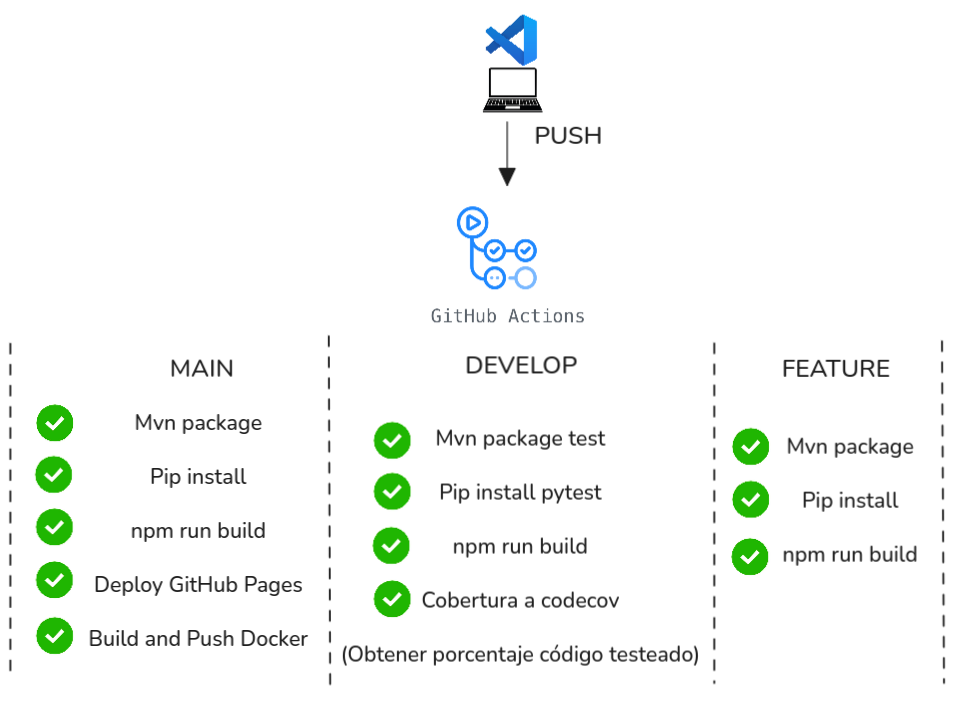
\includegraphics[width=0.8\textwidth]{fotos/githubActions.png}
  \caption{Flujo de desarrollo github actions}
  \label{fig:gitactions}
\end{figure}

\subsubsection*{Workflow para ramas \texttt{feature/*}}

Este workflow se activa con un \texttt{push} a cualquier rama que empiece por \texttt{feature/} y con Pull Requests dirigidos a \texttt{develop}. Las acciones que realiza son: 

\begin{itemize}
  \item Compilación de microservicios en Spring Boot
  \item Instalación de dependencias Python.
  \item Instalación de dependencias Node.js.
  \item Construcción del frontend para validar que no haya errores.
\end{itemize}
\subsubsection*{Workflow para la rama \texttt{develop}}

Este workflow se activa con cada \texttt{push} a la rama \texttt{develop}. Su objetivo principal es ejecutar pruebas automatizadas y medir la cobertura del código. Las acciones que realiza son: 

\begin{itemize}
  \item Configuración del entorno con Ubuntu y Java 17.
  \item Restauración de la caché de dependencias Maven.
  \item Construcción del frontend para validar que no haya errores.
  \item Ejecución de tests en todos los microservicios Java con generación de reportes Jacoco.
  \item Ejecución de tests en Python para microservicios específicos.
  \item Envío de los reportes de cobertura a Codecov \cite{codecov}.
\end{itemize}



\subsubsection*{Workflow para la rama \texttt{main}}

Este workflow se activa al hacer \texttt{push} a la rama \texttt{main} y se centra en realizar el despliegue de la aplicación. Las acciones que realiza son: 

\begin{itemize}
  \item Compilación completa de microservicios Java y construcción de imágenes Docker.
  \item Construcción y despliegue del frontend en GitHub Pages.
  \item Construcción del microservicio en Python.
  \item Login en Docker Hub para subir imágenes Docker de los microservicios Java y Python.
\end{itemize}
\vspace{0.5em}
Además, se ha creado un \href{https://github.com/users/alonsodm12/projects/5}{proyecto en Github}, donde se han definido las historias de usuario y se han organizado en las distintas iteraciones del trabajo. De esta forma, GitHub se ha convertido en la herramienta central para la planificación y el desarrollo.

\begin{figure}[H]
  \centering
  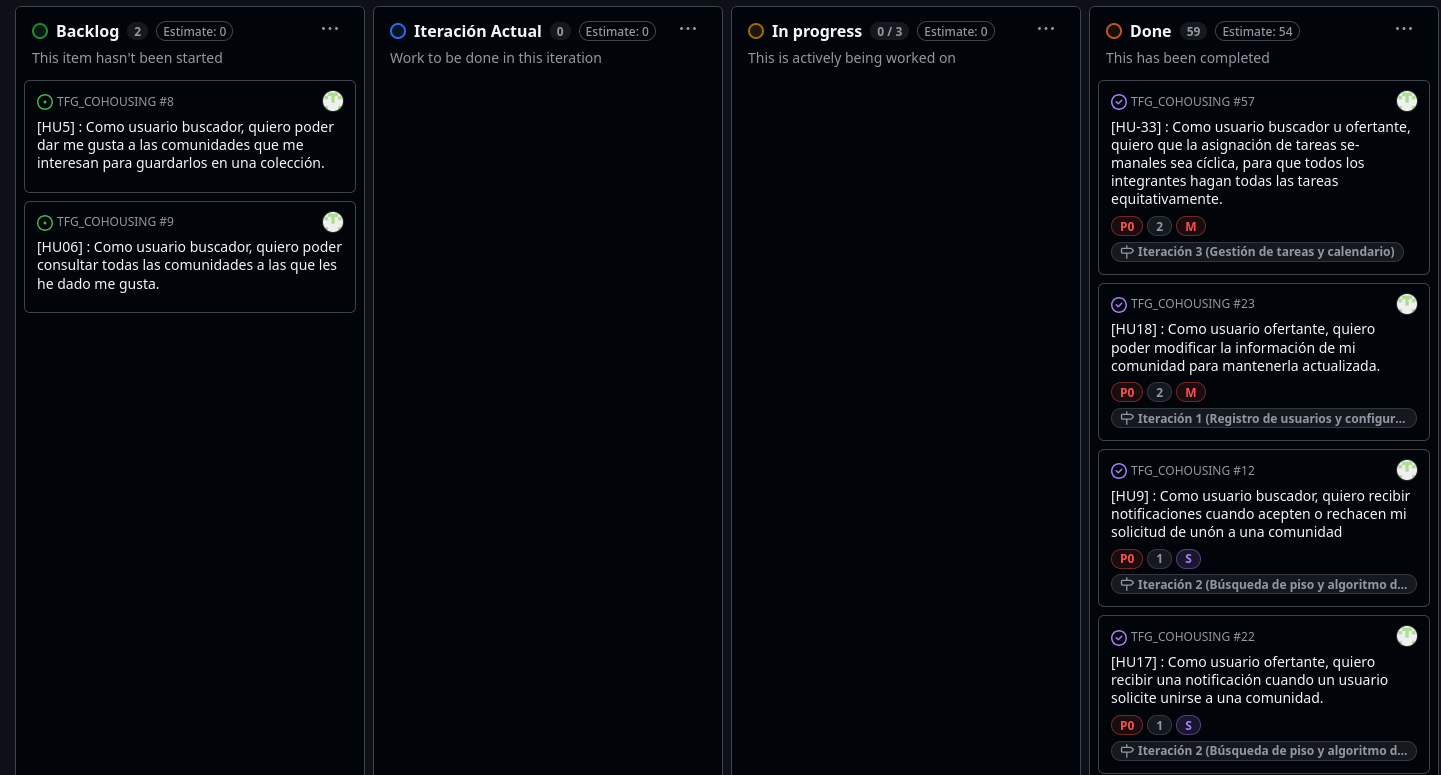
\includegraphics[width=1\textwidth]{fotos/backlog-github.png}
  \caption{Imagen tablero GitHub Project}
\end{figure}

\subsection{Contenerización con Docker}
\begin{figure}[H]
  \centering
  
\includegraphics[width=0.4\textwidth]{fotos/docker.png}
  \caption{Logo docker}
\end{figure}
Cada microservicio y front-end disponen de su propio Dockerfile\cite{docker}, un archivo mediante el cuál se configuran los recursos y dependencias necesarias para su ejecución en un entorno controlado.
Esto permite crear un sistema modular donde cada microservicio se ejecuta de forma aislada en su contenedor específico. 

A continuación se procede a mostrar el ejemplo de configuración de un Dockerfile para los microservicios en Java.
\begin{verbatim}
FROM openjdk:17-jdk-slim
COPY target/demo.jar app.jar
EXPOSE 8081
ENTRYPOINT ["java","-jar","/app.jar"]
\end{verbatim}

Como se puede observar, lo único que se realiza es copiar el .jar del microservicio ya compilado en el contenedor y ejecutarlo. Esta configuración permite desplegar servicios independientes en cualquier entorno compatible con Docker de forma sencilla y efectiva.

\subsection{Orquestación con Docker Compose}

Se emplea un fichero \texttt{docker-compose.yml}\cite{dockercompose} para levantar todo el ecosistema de servicios que componen la aplicación. En general la estructura del archivo es la siguiente
\begin{itemize}
  \item Construcción de microservicios desde sus contextos a partir del DockerFile de cada servicio.
  \item Definición de bases de datos PostgreSQL y servicio RabbitMQ.
  \item Red interna \texttt{cohousing} para comunicación entre contenedores.
  \item Uso de \texttt{depends\_on} para gestionar el orden de arranque.
\end{itemize}

Finalmente para poder ejecutar la aplicación se levanta el entorno completo, esto permite ejecutar en local todos los servicios simultáneamente, para ello se ejecuta el siguiente comando.

\begin{verbatim}
docker-compose up --build
\end{verbatim}

Esta configuración permite una gestión modular, escalable y replicable de la aplicación, facilitando tanto el desarrollo local como el despliegue en entornos de producción.


\section{Funcionalidades clave del sistema}

A continuación se procederá a explicar las diferentes funcionalidades del sistema, mostrando su lógica y flujo de desarrollo.

\subsection{Inicio de sesión y Registro}
Con el objetivo de garantizar la seguridad dentro de la aplicación y asegurar la autenticación y autorización se ha aplicado un sistema de inicio de sesión basado en JWT (JSON Web Token) \cite{jwt}. El flujo de esta funcionalidad es el siguiente: 
 
\begin{itemize}
  \item El usuario envía sus credenciales al \textit{API Gateway}.
  \item El gateway se comunica con el microservicio \textit{Gestión de Usuarios} donde se autentica al usuario y se genera el JWT si las credenciales son correctas.
  \item Este token es enviado al cliente y debe ser adjuntado en el header de las peticiones posteriores para validar la sesión.
  \item En el microservicio \textit{API Gateway}, cada vez que un cliente accede a una ruta protegida, se aplica un filtro personalizado de Spring Security que intercepta la petición y valida la autenticidad del token JWT.
\end{itemize}

\vspace{0.5em}

\begin{figure}[H]
    \centering
    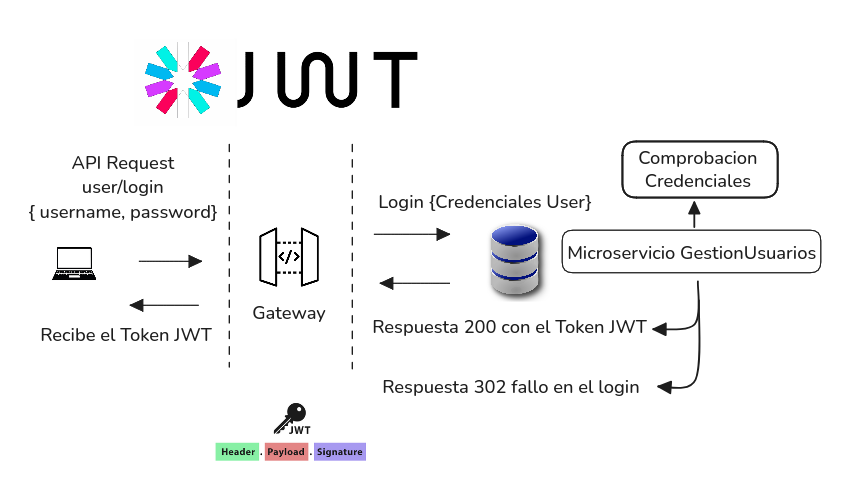
\includegraphics[width=\textwidth]{fotos/jwt_login.png}
    \caption{Flujo de autenticación a través del API Gateway.}
    \label{fig:loginImpl}
\end{figure}

Para implementar el esquema de autenticación basado en JWT representado en la figura \ref{fig:loginImpl}, se han desarrollado los siguientes componentes en la aplicación Spring Boot:
\vspace{0.5em}
\begin{enumerate}[label=\textbf{\arabic*.}]
    \item \textbf{Filtro de seguridad en la API Gateway:} \\
    Se definió un filtro de seguridad que se inserta en la cadena de filtros de Spring Security\cite{springsecurityjwt}. Este filtro es responsable de establecer los requisitos de seguridad correspondientes para cada ruta definida  y de comprobar la validez del token JWT en cada solicitud a una ruta protegida.

    \item \textbf{Generación del token JWT:} \\
    Cuando los datos proporcionados por el usuario durante el proceso de inicio de sesión sean correctos, se procede a generar un token JWT que contiene la información de autenticación del usuario, en nuestro caso el nombre de usuario y el rol.

    \item \textbf{Controlador de autenticación:} \\
    Se definió un controlador REST que gestiona las peticiones de autenticación. Este controlador valida las credenciales del usuario y, en caso de ser válidas, devuelve el token JWT en la respuesta.
\end{enumerate}


\begin{lstlisting}[language=Java, caption={Pseudocódigo del controlador login}]
function login(loginRequestDTO, response):

    try:
        # Intentar autenticar al usuario
        token = authService.login(loginRequestDTO)

        # Guardar el token como cookie de autenticacion
        addAuthCookie(response, token)

        # Obtener el rol del usuario desde el token
        role = tokenService.getRoleFromToken(token)

        # Devolver respuesta de exito con datos del usuario
        return ResponseEntity.ok({
            "message": "Login correcto",
            "username": loginRequestDTO.username,
            "role": role
        })

    except AuthenticationException:
        # Si las credenciales no son validas, devolver error
        return ResponseEntity.status(BAD_REQUEST).body({
            "error": "Credenciales invalidas"
        })
\end{lstlisting}

En el frontend simplemente se rellena el formulario de inicio de sesión, mostrado en la figura \ref{fig:loginFront}, enviándo los datos necesarios para la autenticación.
\begin{figure}[H]
  \centering
  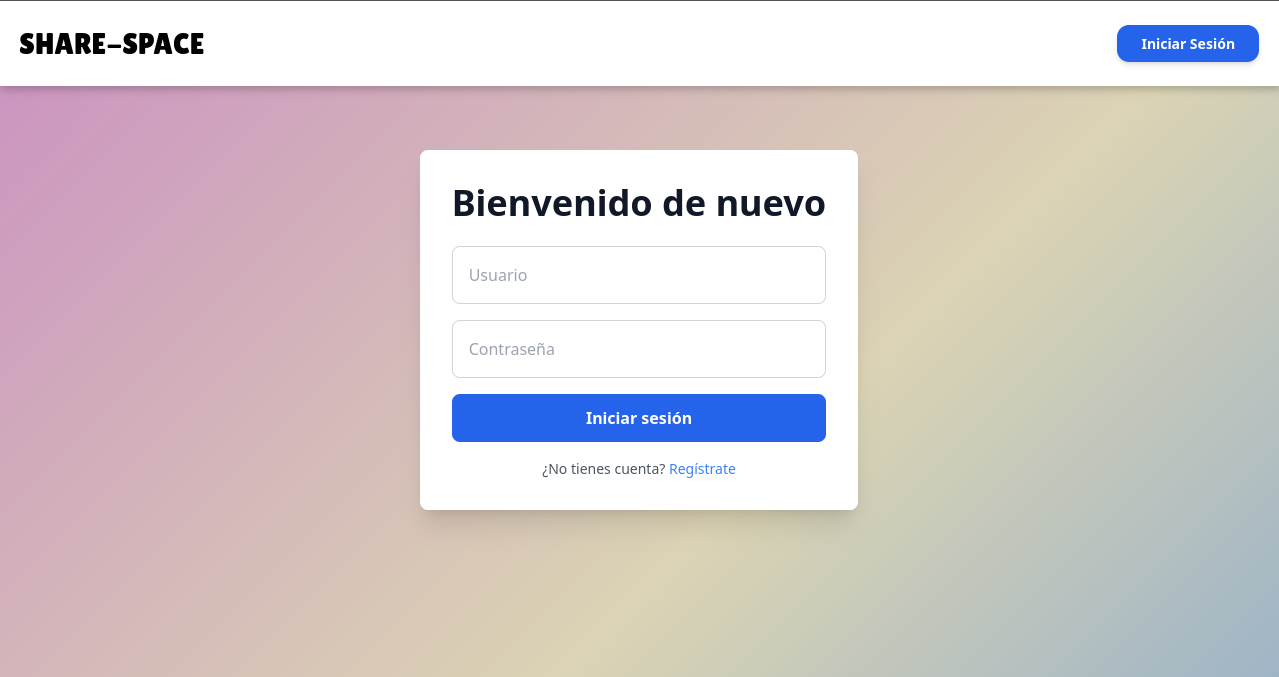
\includegraphics[width=1\textwidth]{fotos/login.png}
  \caption{Pantalla del login en el front-end}
  \label{fig:loginFront}
\end{figure}


\subsection{Comunicación Asíncrona entre Microservicios}

Para garantizar la resiliencia e independencia entre los distintos microservicios que componen el sistema, es fundamental que la comunicación entre ellos sea asíncrona ya que de otra forma podrían producirse cuellos de botella o incluso una caída del sistema entero ante algún fallo en uno de los servicios.
Con el objetivo de implementar este tipo de comunicación, se ha integrado el broker de mensajería asíncrona \textbf{RabbitMQ}, que actúa como intermediario en el intercambio de mensajes entre microservicios.

\subsection*{Flujo de comunicación}

El flujo seguido para establecer esta arquitectura de mensajería es el siguiente:

\begin{itemize}
    \item Los microservicios publican eventos en colas específicas gestionadas por RabbitMQ.
    \item Otros microservicios se suscriben a dichas colas, reaccionando ante los mensajes recibidos.
    \item Esta arquitectura permite reducir el acoplamiento entre los microservicios, consiguiendo una mayor escalabilidad, tolerancia a fallos e independencia entre ellos.
\end{itemize}

\subsection*{Funcionamiento del sistema}

La lógica general de funcionamiento se basa en los siguientes pasos:

\begin{enumerate}[label=\textbf{\arabic*.}]
    \item El microservicio define un evento que producirá una comunicación con otro microservicio, por ejemplo solicitar la unión a una comunidad.
    \item El microservicio productor registra una nueva cola específica en RabbitMQ que estará asociada al evento definido anteriormente.
    \item Al producirse el evento, se crea un mensaje con los datos relevantes y se publica en dicha cola.
    \item Los microservicios consumidores definen \textit{listeners} (funciones observadoras) que se mantienen a la escucha.
    \item Cuando el mensaje llega a la cola correspondiente, el \textit{listener} lo recibe, extrae los datos y ejecuta una lógica específica en respuesta al evento.
\end{enumerate}

Este patrón de comunicación mostrado en la figura \ref{fig:rabbitmqexpl} favorece un diseño desacoplado, reactivo y preparado para entornos distribuidos y de alta disponibilidad.

\begin{figure}[h!]
  \centering
  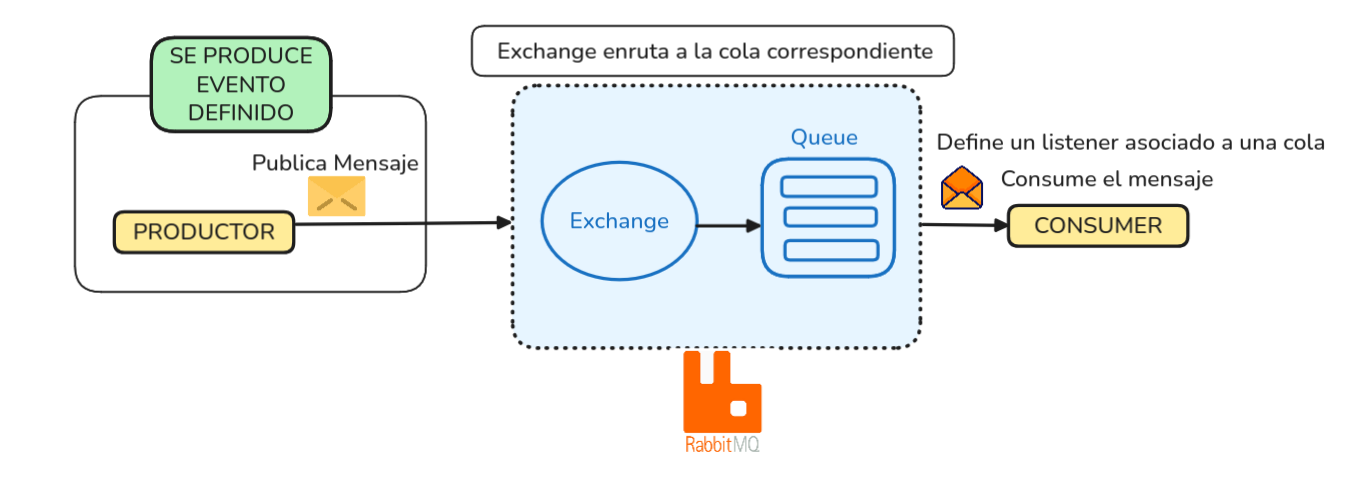
\includegraphics[width=1\textwidth]{fotos/rabbitmqexpl.png}
  \caption{Flujo de eventos y comunicación entre microservicios usando RabbitMQ}
  \label{fig:rabbitmqexpl}
\end{figure}
\subsection{Recomendación de Comunidades}

Toda la lógica e implementación relacionada con la recomendación de comunidades se ha encapsulado en un microservicio independiente denominado \textbf{Recomendaciones}. Esta decisión se basa en que el módulo presenta suficientes reglas de negocio como para ser considerado una entidad lógica separada dentro del sistema.

\vspace{0.5em}
Para la implementación del microservicio se ha utilizado el lenguaje de programación \textbf{Python}, apoyado en las siguientes bibliotecas:

\begin{itemize}
    \item \texttt{Pandas} \cite{pandas}, para el tratamiento y análisis de datos.
    \item \texttt{FastAPI} \cite{fastapi}, para la creación y estructuración de la API REST.
\end{itemize}

\subsection*{Algoritmo de recomendación}

Con el objetivo de conseguir una recomendación personaliza para cada usuario se ha seguido un enfoque basado en técnicas de \textit{clustering}, mediante el algoritmo \textbf{K-Means} \cite{kmeans}. Esto ha permitido agrupar las comunidades en función de la similitud de sus parámetros de afinidad. Una vez organizados estos grupos, se ha identificado el más cercano al usuario calculando la similitud entre los valores de afinidad del usuario y los de las comunidades de cada grupo. La lógica general del sistema se puede resumir del siguiente modo:


\vspace{0.5em}
\begin{itemize}
    \item Las comunidades se agrupan en \textit{clusters} en función de sus características individuales (afinidad, sociabilidad, limpieza, etc.).
    \item Se entrena un modelo \texttt{KMeans} únicamente con las comunidades.
    \item Se predice a qué \textit{cluster} pertenecería un usuario en base a sus características.
    \item Se seleccionan las comunidades que pertenecen al mismo \textit{cluster} que el usuario.
    \item Se ordenan esas comunidades según su cercanía al vector escalado del usuario, de forma que sea lo más personalizado posible.
\end{itemize}

\subsection*{Procedimiento de recomendación}

Dentro del propio microservicio se ha seguido el siguiente flujo para generar las recomendaciones personalizadas para cada usuario:

\begin{enumerate}[label=\textbf{\arabic*.}]
    \item Se recuperan los datos del usuario objetivo y de las comunidades desde sus respectivas bases de datos.
    \item Se normalizan los parámetros de afinidad tanto del usuario como de las comunidades, esto es necesario para que la distancia euclídea tenga sentido.
    \item Se entrena un modelo de \texttt{K-Means} con los datos escalados de las comunidades.
    \item Se predice a qué \textit{cluster} pertenecería el usuario, para ello se calcula la diferencia (distancia euclídea) entre el vector del usuario y el centroide de cada grupo, que funciona como representación del perfil idea de ese grupo de comunidades.
    \item Se calcula la distancia euclídea entre cada comunidad del mismo \textit{cluster} escogido y el vector escalado del usuario.
    \item Se transforma la distancia en un porcentaje de afinidad (0 a 100).
    \item Las comunidades del clúster se ordenan por mayor afinidad y se seleccionan las \texttt{n} más afines para formar la recomendación.
\end{enumerate}
\vspace{0.5em}

\begin{lstlisting}[language=Python, caption={Pseudocódigo de la función recommend\_communities\_by\_user}]
def recommend_communities_by_user(user, communities, n_recommendations=10):
    
    # Si no hay comunidades, devolvemos la lista vacia
    if communities is None or len(communities) == 0:
        return []

    # Preprocesar y escalar datos, es necesario tener los datos escalados y en un formato correcto para aplicar K-Means
    user_scaled, communities_scaled = preprocess_data(user, communities)

    #Si no hay usuarios, devolvemos error
    if user_scaled is None or communities_scaled is None:
        raise ValueError("Error al escalar los datos")

    # Definimos el numero de clusters que tendremos
    n_clusters = min(3, len(communities_scaled))
    if n_clusters == 0:
        return []

    # Entrenar modelo KMeans
    kmeans = KMeans(n_clusters=n_clusters, random_state=42)
    kmeans.fit(communities_scaled)

    # Predecir cluster del usuario y de las comunidades

    # K-Means nos dice a que cluster pertenece el usuario
    user_cluster = kmeans.predict(user_scaled)[0]

    # K-Means predice en que cluster cae cada comunidad
    # Devuelve un vector indicando en que cluster se encuentra cada comunidad
    communities_clusters = kmeans.predict(communities_scaled)

    # Calculamos el centroide del cluster del usuario
    # El centroide es un vector con las coordenadas medias de ese grupo
    user_center = kmeans.cluster_centers_[user_cluster]

    # Calcular distancias entre las comunidades del cluster escogido y el centroide del usuario
    distances = []
    # Recorremos todas las comunidades
    for i, community_scaled in enumerate(communities_scaled):
        # Solo nos fijamos en aquellas que estan en el mismo cluster que el usuario
        if communities_clusters[i] == user_cluster:
            # Se calcula la distancia euclidea (np.linalg.norm(...)) entre la comunidad[i} y el usuario
            dist = distancia_euclidiana(community_scaled, user_scaled[0])
            #Esto devuelve una lista de pares indicando primero el id de la comunidad y segundo un valor
            #que indica que tan lejos estan de el
            distances.append((i, dist))

    if not distances:
        return []

    # Normalizar distancias para calcular afinidad
    max_distance = max(dist for _, dist in distances)
    if max_distance == 0:
        max_distance = 1

    MIN_AFFINITY = 30
    affinities = []
    for i, dist in distances:
        if dist es finita:
            affinity = 100 * (1 - dist / max_distance)
        else:
            affinity = 0
        # Limitar entre MIN_AFFINITY y 100
        affinity = max(min(affinity, 100), MIN_AFFINITY)
        affinities.append((i, round(affinity)))

    # Ordenar comunidades por afinidad descendente
    affinities.sort(descending by affinity)

    # Construir lista final de recomendaciones
    recommended = []
    for i, affinity in affinities[:n_recommendations]:
        recommended.append(
            community_to_dict(communities[i]) + {"affinity": affinity}
        )

    return recommended
\end{lstlisting}



Este enfoque permite recomendar comunidades al usuario de forma personalizada y priorizando la afinidad entre ambos.

\begin{figure}[H]
  \centering
  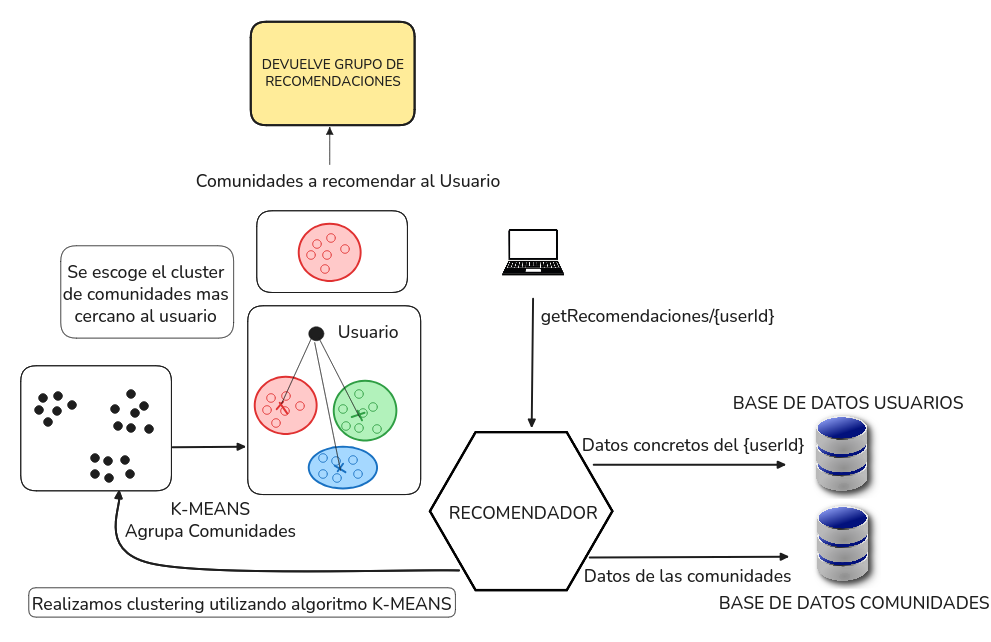
\includegraphics[width=1\textwidth]{fotos/clustering.png}
  \caption{Explicación del sistema de recomendación para usuarios}
  \label{fig:clustering}
\end{figure}
Este sistema de recomendación mostrado en la figura \ref{fig:clustering} es especialmente útil en escenarios de \textit{cold start}, ya que no requiere un historial de interacciones del usuario, sino que se basa en similitud de perfiles.
Cabe destacar que la aplicación permite refinar aún más las recomendaciones de comunidades mediante filtros adicionales, como la distancia al usuario y el rango de precio. Esto proporciona una lista de comunidades más personalizada y ajustada a las preferencias del usuario.

Finalmente, tal como se observa en la figura \ref{fig:frontend-recomendador}, el usuario dispone de opciones para aplicar filtros adicionales y se le muestran las comunidades recomendadas junto a sus datos más representativos.
\vspace{0.5em}
\begin{figure}[H]
  \centering
  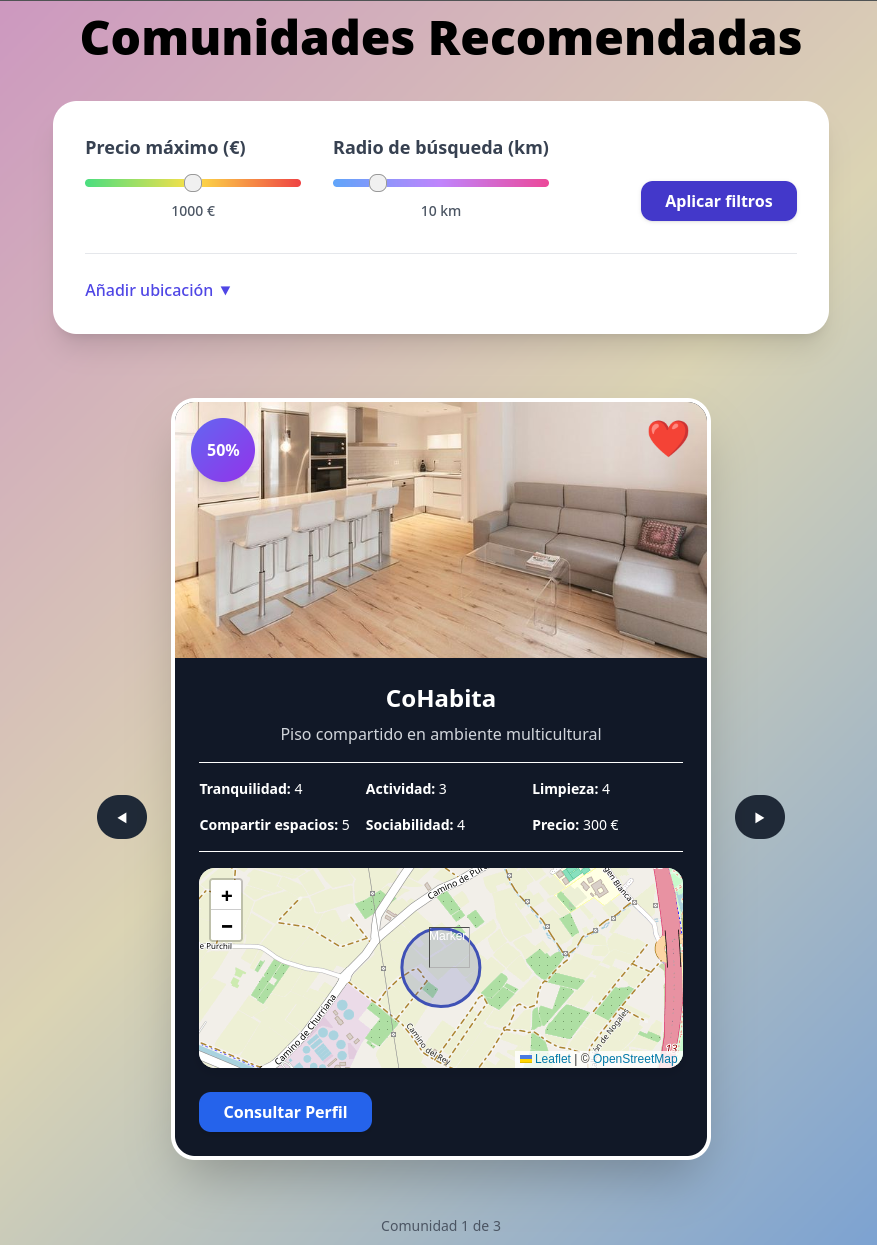
\includegraphics[width=0.8\textwidth]{fotos/frontend-recomendador.png}
  \caption{Pantalla de recomendaciones en el front-end}
  \label{fig:frontend-recomendador}
\end{figure}

\subsection{Proceso de Unión a una Comunidad}

El proceso de unión de un usuario a una comunidad involucra la interacción de varios de los microservicios que componen el sistema, entre ellos los microservicios de \textit{Comunidad}, \textit{Solicitudes} y \textit{GestionUsuarios}.
Para la comunicación entre dichos microservicios se usará como broker RabittMQ \cite{rabbitmq}. El flujo para realizar esta operación dentro del sistema es el siguiente:

\vspace{0.5em}
\begin{enumerate}
  \item El usuario solicita unirse a una comunidad a través de la llamada al endpoint unirse-comunidad del microservicio \textit{GestionComunidades}.
  \item Este microservicio genera un evento y lo publica en RabbitMQ.
  \item El microservicio de \textit{Solicitudes} escucha el evento, registra la solicitud y la notifica al administrador de la comunidad.
  \item El administrador puede aceptar o rechazar la solicitud mediante el microservicio de \textit{Solicitudes}. Al aceptar o rechazar el microservicio genera un evento y lo publica en RabbitMQ
  \item El microservicio de \textit{GestionComunidades} escucha el evento y si el administrador ha aceptado, une al usuario a la comunidad. Finalmente este microservicio emite un evento y lo publica en RabbitMQ.
  \item El microservicio de \textit{Solicitudes} escucha el evento, registra la respuesta y la notifica al usuario buscador.
\end{enumerate}

\vspace{0.5em}

Este flujo de comunicación entre los diferentes microservicios queda resumido en la figura \ref{fig:union-comunidad}, mostrando como los diferentes microservicios van generando eventos en función del estado de la comunicación actual y como todo el proceso es orquestado por RabbitMQ.

\begin{figure}[H]
  \centering
  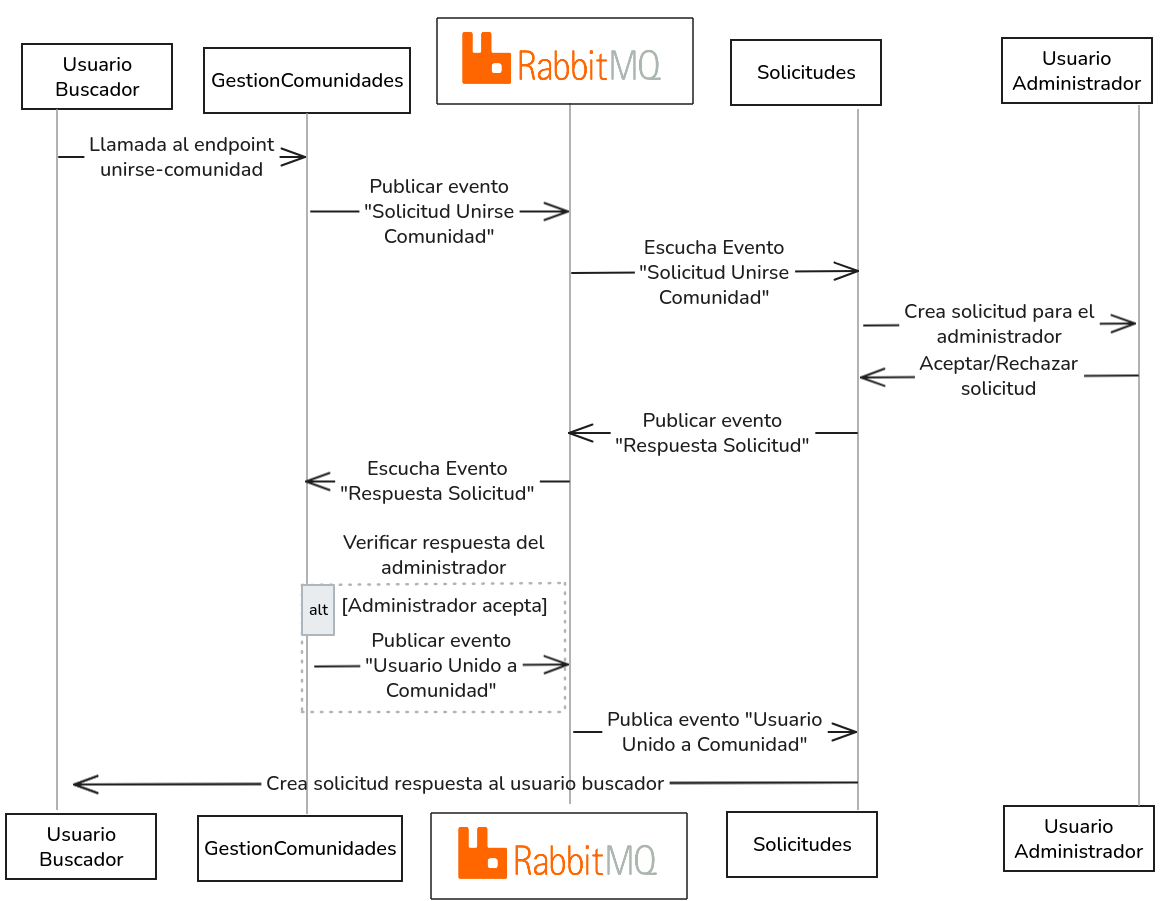
\includegraphics[width=1\textwidth]{fotos/usuarioUneComunidad.png}
  \caption{Esquema del flujo para la unión de un usuario a una comunidad}
  \label{fig:union-comunidad}
\end{figure}





\newpage


\subsection{Gestión de comunidades}
El microservicio de \textbf{Gestión de Comunidades} encapsula el mayor volumen de lógica de negocio dentro del sistema, siendo responsable de coordinar todos los aspectos relacionados con las comunidades: sus eventos, la asignación y la gestión de tareas.

Entre las funcionalidades más relevantes implementadas en este servicio, destacan:

\begin{itemize}
  \item \textbf{Reparto automático de tareas:}  
  El sistema realiza una distribución automática de las tareas entre los usuarios que forman parte de una comunidad, siguiendo un orden cíclico. Este reparto se ejecuta de forma semanal, asegurando así un equilibrio en la carga de trabajo entre los miembros.

  \item \textbf{Administración de tareas por parte del usuario:}  
  Los usuarios tienen la posibilidad de consultar y reorganizar sus tareas mediante una interfaz de calendario interactivo. Esta herramienta permite una gestión más intuitiva y visual de sus responsabilidades.
\end{itemize}

\subsection*{Reparto Automático de Tareas}

El reparto automático de tareas tiene como objetivo asegurar una distribución equitativa del trabajo entre los miembros de cada comunidad. Para ello, se sigue un algoritmo cíclico que asigna las tareas disponibles a los usuarios de manera rotativa.

Con este objetivo en mente se ha diseñado el siguiente algoritmo teniendo en cuenta:
\begin{itemize}
  \item El conjunto de usuarios activos en la comunidad.
  \item Las tareas asociadas a la comunidad.
  \item El historial de asignaciones anteriores, para mantener el reparto equitativo.
\end{itemize}

De esta manera, el sistema garantiza una planificación justa y eficiente, mejorando la organización interna de cada comunidad.

\subsection*{Lógica del reparto cíclico}

El reparto de tareas se ha diseñado siguiendo una lógica sencilla pero equitativa. A continuación, se describe el comportamiento implementado:

\begin{itemize}
    \item Las tareas se distribuyen de forma \textbf{cíclica} entre los integrantes de la comunidad. De este modo, con el tiempo, todos los miembros participarán en todas las tareas.
    \item Al crear una nueva tarea, se define el \textbf{número de participantes requeridos}.
    \item En el primer reparto, se asignan por defecto los primeros usuarios disponibles. De forma que, si hay cuatro tareas y tres miembros, se asignará la primera tarea al primer miembro; la segunda, al segundo y así sucesivamente en orden cíclico.
    \item En repartos sucesivos, se utiliza un índice rotativo almacenado en la comunidad para determinar desde qué usuario comenzar la asignación. Este índice se va actualizando con cada tarea para que todos los usuarios participen proporcionalmente en alguna tarea en cada iteración. Si un nuevo usuario se une a la comunidad, se incorpora automáticamente a la lista de usuarios rotativos.
\end{itemize}

\vspace{0.25em}
Para lograr la ejecución de forma semanal del reparto se ha utilizado la anotación \textit{@Scheduled(cron = )}. Con esta anotación podemos ejecutar este método definido en el backend de forma periódica; en nuestro caso cada semana.
\begin{lstlisting}[language=Python, caption={Pseudocódigo de la función repartirTareasSemanalmente}]
@Scheduled(cron = "0 0 23 * * SUN")
@Transactional
def void repartirTareasSemanalmente():
    # Obtener todas las comunidades
    comunidades = obtenerTodasLasComunidades()
    hoy = fechaActual()
    # Iterar sobre cada comunidad
    for comunidad in comunidades:
        
        # Repartir tareas de forma ciclica
        repartirTareasCiclico(comunidad.id)
        
        # Generar resumen semanal
        generarResumenSemanal(comunidad, hoy)

        # Obtener lista de identificadores de usuarios de la comunidad
        idUsuarios = lista(comunidad.integrantes)

        # Crear notificacion de reparto de tareas
        payload = crearNotificacionReparto(
            comunidad.id,
            comunidad.nombre,
            "Se ha realizado el reparto de tareas en tu comunidad",
            idUsuarios
        )

        # Enviar notificacion a la cola de mensajeria (RabbitMQ)
        enviarMensajeCola(
            EXCHANGE_REPARTO_TAREAS,
            ROUTING_KEY_REPARTO_TAREAS,
            payload
        )

\end{lstlisting}
\subsection*{Notificación y visualización}

Para asegurar que los usuarios estén al tanto de sus tareas, el sistema emite notificaciones cuando se realiza el reparto semanal:

\begin{itemize}
    \item De manera semanal se emite una \textbf{notificación automática a todos los integrantes de la comunidad} de forma que se les avise del nuevo reparto. Esto se implementa con la definición de un evento dentro de la función de reparto semanal que es gestionada por RabbitMQ. 
\end{itemize}


A continuación pasamos a comentar la Administración de tareas por parte del usuario.
\vspace{0.5em}
\subsection{Administración de Tareas por Parte de los Usuarios}

Con el objetivo de facilitar la administración de tareas dentro de la comunidad, se ha desarrollado una interfaz interactiva que permite a los usuarios visualizar, asignar y reprogramar sus tareas mediante un calendario dinámico.

Buscando la mejor experiencia de usuario posible, se ha implementado una funcionalidad de \textit{drag and drop} (arrastrar y soltar), que permite al usuario mover las tareas a diferentes franjas horarias en el calendario, asignándoles así una fecha y hora de inicio de forma intuitiva.

El flujo de funcionamiento del componente es el siguiente:

\vspace{0.5em}
\begin{enumerate}
  \item \textbf{Carga de las tareas del usuario:}  
  En primer lugar, se obtienen todas las tareas correspondientes al usuario mediante el \textit{endpoint} \texttt{/tareas/{idUsuario}}.  
  \begin{itemize}
    \item Las tareas que no tienen fecha asignada se muestran en una columna lateral para ser planificadas por el usuario.
    \item Las tareas ya planificadas se adaptan al formato requerido por la biblioteca \texttt{FullCalendar} \cite{fullcalendar-docs}(\texttt{id}, \texttt{title}, \texttt{start}) y se representan directamente en el calendario.
  \end{itemize}

  \item \textbf{Funcionalidad Drag and Drop:}  
  Las tareas sin fecha se convierten en elementos arrastrables mediante la clase \texttt{Draggable} de \texttt{FullCalendar}. Esto permite al usuario arrastrar una tarea desde la columna lateral y soltarla en una franja del calendario.

  \item \textbf{Asignación de fecha al soltar la tarea:}  
  Cuando el usuario suelta una tarea sobre el calendario, se ejecuta el método \texttt{handleReceive}. Este método extrae el \texttt{id} de la tarea y la fecha seleccionada, y envía esta información al \texttt{backend} mediante el método \texttt{updateTarea} para registrar la nueva fecha.

  \item \textbf{Reprogramación de tareas:}  
  Si el usuario mueve una tarea ya planificada a una nueva franja horaria dentro del calendario, se ejecuta el método \texttt{handleEventDrop}, el cual recalcula la nueva fecha y la actualiza en el \texttt{backend}.
\end{enumerate}
\newpage
\begin{lstlisting}[language=Java, caption={Pseudocódigo de tareas drag and drop y asignacion fecha al soltar tarea}]
function drag and drop(tareasSinFecha):

    # Obtener el elemento contenedor de tareas externas
    draggableEl = getElementById("external-tasks")

    # Verificar si existe y si aun no ha sido inicializado
    if draggableEl != null AND draggableEl._draggableInitialized == false:

        # Crear un nuevo objeto Draggable sobre el contenedor
        # De esta forma todo lo contenido en el contenedor con item fc-task es arrastrable
        new Draggable(draggableEl, {
            itemSelector: ".fc-task",
            eventData: (el) => {
                id = el.getAttribute("data-id") OR ""
                title = el.getAttribute("data-title") OR el.textContent OR ""
                return { id, title }
            }
        })

        # Marcar el elemento como inicializado
        draggableEl._draggableInitialized = true


function asignacion fecha al soltar tarea(info):
    # Esta funcion se ejecuta cada vez que se suelta una tarea en una celda del calendario 

    # Obtener id de la tarea arrastrada
    id = info.event.id

    # Calcular la nueva fecha con ajuste de +2 horas
    if info.event.start != null:
        fecha = toISOString(info.event.start + 2 horas).slice(0,19)
    else:
        fecha = ""

    try:
        # Actualizar fecha de la tarea en el backend
        updateDateTarea(id, fecha)

        # Eliminar la tarea de la lista sin fecha
        setTareasSinFecha( tareasSinFecha.filter(t -> t.id != id) )

        # Agregar la tarea a la lista con fecha
        setTareasConFecha( tareasConFecha + { id, title: info.event.title, start: fecha })

    catch error:
        # En caso de error revertir el drag and drop
        log(error)
        info.revert()
\end{lstlisting}

Gracias a esta implementación, se ha creado una vista de administración de tareas (figura \ref{fig:admin-tareas}) que permite al usuario gestionarlas de forma dinámica. Desde esta interfaz se puede tanto planificar las tareas por primera vez como reorganizarlas posteriormente.
\begin{figure}[h!]
  \centering
  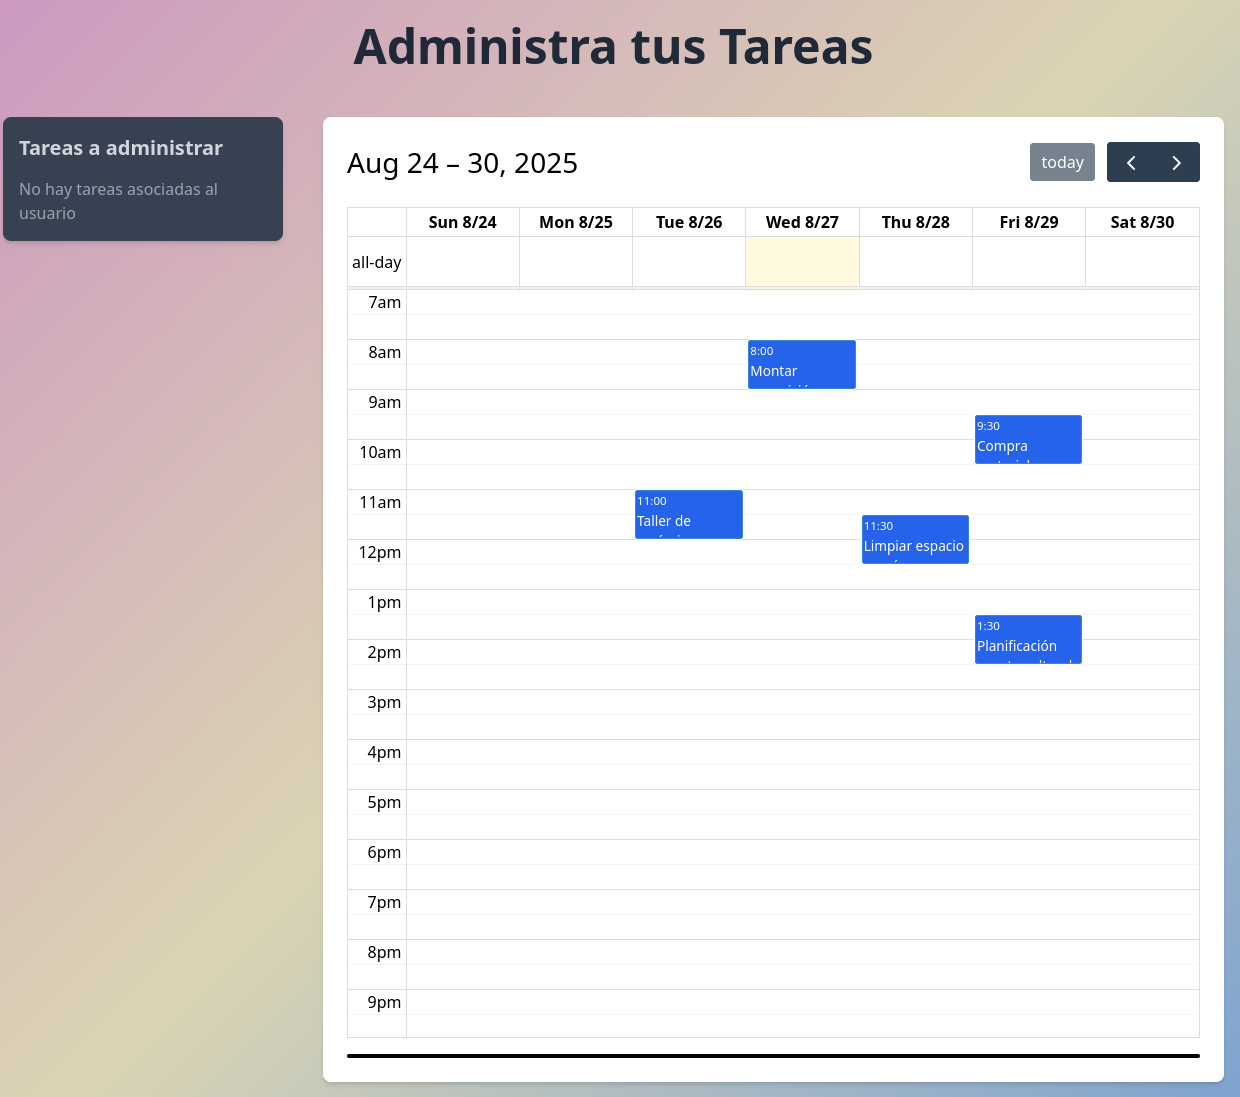
\includegraphics[width=1\textwidth]{fotos/admi-tareas.png}
  \caption{Vista del usuario para la administración de tareas dinámicamente}
  \label{fig:admin-tareas}
\end{figure}